\documentclass[]{article}
\usepackage{lmodern}
\usepackage{amssymb,amsmath}
\usepackage{ifxetex,ifluatex}
\usepackage{fixltx2e} % provides \textsubscript
\ifnum 0\ifxetex 1\fi\ifluatex 1\fi=0 % if pdftex
  \usepackage[T1]{fontenc}
  \usepackage[utf8]{inputenc}
\else % if luatex or xelatex
  \ifxetex
    \usepackage{mathspec}
  \else
    \usepackage{fontspec}
  \fi
  \defaultfontfeatures{Ligatures=TeX,Scale=MatchLowercase}
\fi
% use upquote if available, for straight quotes in verbatim environments
\IfFileExists{upquote.sty}{\usepackage{upquote}}{}
% use microtype if available
\IfFileExists{microtype.sty}{%
\usepackage{microtype}
\UseMicrotypeSet[protrusion]{basicmath} % disable protrusion for tt fonts
}{}
\usepackage[margin=1in]{geometry}
\usepackage{hyperref}
\hypersetup{unicode=true,
            pdftitle={Project},
            pdfauthor={Farbod Taymouri},
            pdfborder={0 0 0},
            breaklinks=true}
\urlstyle{same}  % don't use monospace font for urls
\usepackage{color}
\usepackage{fancyvrb}
\newcommand{\VerbBar}{|}
\newcommand{\VERB}{\Verb[commandchars=\\\{\}]}
\DefineVerbatimEnvironment{Highlighting}{Verbatim}{commandchars=\\\{\}}
% Add ',fontsize=\small' for more characters per line
\usepackage{framed}
\definecolor{shadecolor}{RGB}{248,248,248}
\newenvironment{Shaded}{\begin{snugshade}}{\end{snugshade}}
\newcommand{\KeywordTok}[1]{\textcolor[rgb]{0.13,0.29,0.53}{\textbf{#1}}}
\newcommand{\DataTypeTok}[1]{\textcolor[rgb]{0.13,0.29,0.53}{#1}}
\newcommand{\DecValTok}[1]{\textcolor[rgb]{0.00,0.00,0.81}{#1}}
\newcommand{\BaseNTok}[1]{\textcolor[rgb]{0.00,0.00,0.81}{#1}}
\newcommand{\FloatTok}[1]{\textcolor[rgb]{0.00,0.00,0.81}{#1}}
\newcommand{\ConstantTok}[1]{\textcolor[rgb]{0.00,0.00,0.00}{#1}}
\newcommand{\CharTok}[1]{\textcolor[rgb]{0.31,0.60,0.02}{#1}}
\newcommand{\SpecialCharTok}[1]{\textcolor[rgb]{0.00,0.00,0.00}{#1}}
\newcommand{\StringTok}[1]{\textcolor[rgb]{0.31,0.60,0.02}{#1}}
\newcommand{\VerbatimStringTok}[1]{\textcolor[rgb]{0.31,0.60,0.02}{#1}}
\newcommand{\SpecialStringTok}[1]{\textcolor[rgb]{0.31,0.60,0.02}{#1}}
\newcommand{\ImportTok}[1]{#1}
\newcommand{\CommentTok}[1]{\textcolor[rgb]{0.56,0.35,0.01}{\textit{#1}}}
\newcommand{\DocumentationTok}[1]{\textcolor[rgb]{0.56,0.35,0.01}{\textbf{\textit{#1}}}}
\newcommand{\AnnotationTok}[1]{\textcolor[rgb]{0.56,0.35,0.01}{\textbf{\textit{#1}}}}
\newcommand{\CommentVarTok}[1]{\textcolor[rgb]{0.56,0.35,0.01}{\textbf{\textit{#1}}}}
\newcommand{\OtherTok}[1]{\textcolor[rgb]{0.56,0.35,0.01}{#1}}
\newcommand{\FunctionTok}[1]{\textcolor[rgb]{0.00,0.00,0.00}{#1}}
\newcommand{\VariableTok}[1]{\textcolor[rgb]{0.00,0.00,0.00}{#1}}
\newcommand{\ControlFlowTok}[1]{\textcolor[rgb]{0.13,0.29,0.53}{\textbf{#1}}}
\newcommand{\OperatorTok}[1]{\textcolor[rgb]{0.81,0.36,0.00}{\textbf{#1}}}
\newcommand{\BuiltInTok}[1]{#1}
\newcommand{\ExtensionTok}[1]{#1}
\newcommand{\PreprocessorTok}[1]{\textcolor[rgb]{0.56,0.35,0.01}{\textit{#1}}}
\newcommand{\AttributeTok}[1]{\textcolor[rgb]{0.77,0.63,0.00}{#1}}
\newcommand{\RegionMarkerTok}[1]{#1}
\newcommand{\InformationTok}[1]{\textcolor[rgb]{0.56,0.35,0.01}{\textbf{\textit{#1}}}}
\newcommand{\WarningTok}[1]{\textcolor[rgb]{0.56,0.35,0.01}{\textbf{\textit{#1}}}}
\newcommand{\AlertTok}[1]{\textcolor[rgb]{0.94,0.16,0.16}{#1}}
\newcommand{\ErrorTok}[1]{\textcolor[rgb]{0.64,0.00,0.00}{\textbf{#1}}}
\newcommand{\NormalTok}[1]{#1}
\usepackage{graphicx,grffile}
\makeatletter
\def\maxwidth{\ifdim\Gin@nat@width>\linewidth\linewidth\else\Gin@nat@width\fi}
\def\maxheight{\ifdim\Gin@nat@height>\textheight\textheight\else\Gin@nat@height\fi}
\makeatother
% Scale images if necessary, so that they will not overflow the page
% margins by default, and it is still possible to overwrite the defaults
% using explicit options in \includegraphics[width, height, ...]{}
\setkeys{Gin}{width=\maxwidth,height=\maxheight,keepaspectratio}
\IfFileExists{parskip.sty}{%
\usepackage{parskip}
}{% else
\setlength{\parindent}{0pt}
\setlength{\parskip}{6pt plus 2pt minus 1pt}
}
\setlength{\emergencystretch}{3em}  % prevent overfull lines
\providecommand{\tightlist}{%
  \setlength{\itemsep}{0pt}\setlength{\parskip}{0pt}}
\setcounter{secnumdepth}{0}
% Redefines (sub)paragraphs to behave more like sections
\ifx\paragraph\undefined\else
\let\oldparagraph\paragraph
\renewcommand{\paragraph}[1]{\oldparagraph{#1}\mbox{}}
\fi
\ifx\subparagraph\undefined\else
\let\oldsubparagraph\subparagraph
\renewcommand{\subparagraph}[1]{\oldsubparagraph{#1}\mbox{}}
\fi

%%% Use protect on footnotes to avoid problems with footnotes in titles
\let\rmarkdownfootnote\footnote%
\def\footnote{\protect\rmarkdownfootnote}

%%% Change title format to be more compact
\usepackage{titling}

% Create subtitle command for use in maketitle
\providecommand{\subtitle}[1]{
  \posttitle{
    \begin{center}\large#1\end{center}
    }
}

\setlength{\droptitle}{-2em}

  \title{Project}
    \pretitle{\vspace{\droptitle}\centering\huge}
  \posttitle{\par}
    \author{Farbod Taymouri}
    \preauthor{\centering\large\emph}
  \postauthor{\par}
    \date{}
    \predate{}\postdate{}
  

\begin{document}
\maketitle

\section{Introduction}\label{introduction}

The following libraries will be used in this project.

\begin{Shaded}
\begin{Highlighting}[]
\KeywordTok{library}\NormalTok{(astsa)}
\KeywordTok{library}\NormalTok{(ggplot2)}
\KeywordTok{library}\NormalTok{(forecast)}
\KeywordTok{library}\NormalTok{(dynlm)}
\KeywordTok{library}\NormalTok{(xts)}
\KeywordTok{library}\NormalTok{(corrplot)}
\KeywordTok{library}\NormalTok{(psych)}
\end{Highlighting}
\end{Shaded}

\section{Dataset description}\label{dataset-description}

The dataset used in this project is about
\href{https://archive.ics.uci.edu/ml/datasets/Appliances+energy+prediction}{Appliances
energy prediction Data Set} that is available on UCI website. The data
set is at 10 min for about 4.5 months. The house temperature and
humidity conditions were monitored with a ZigBee wireless sensor
network. Each wireless node transmitted the temperature and humidity
conditions around 3.3 min. Then, the wireless data was averaged for 10
minutes periods. The energy data was logged every 10 minutes with m-bus
energy meters. Weather from the nearest airport weather station
(Chievres Airport, Belgium) was downloaded from a public data set from
Reliable Prognosis (rp5.ru), and merged together with the experimental
data sets using the date and time column. Two random variables have been
included in the data set for testing the regression models and to filter
out non predictive attributes (parameters).

\subsection{Attributes}\label{attributes}

The following attributes are used in this dataset:

\begin{itemize}
\tightlist
\item
  date time year-month-day hour:minute:second
\item
  Appliances, energy use in Wh
\item
  lights, energy use of light fixtures in the house in Wh
\item
  T1, Temperature in kitchen area, in Celsius
\item
  RH\_1, Humidity in kitchen area, in \%
\item
  T2, Temperature in living room area, in Celsius
\item
  RH\_2, Humidity in living room area, in \%
\item
  T3, Temperature in laundry room area
\item
  RH\_3, Humidity in laundry room area, in \%
\item
  T4, Temperature in office room, in Celsius
\item
  RH\_4, Humidity in office room, in \%
\item
  T5, Temperature in bathroom, in Celsius
\item
  RH\_5, Humidity in bathroom, in \%
\item
  T6, Temperature outside the building (north side), in Celsius
\item
  RH\_6, Humidity outside the building (north side), in \%
\item
  T7, Temperature in ironing room , in Celsius
\item
  RH\_7, Humidity in ironing room, in \%
\item
  T8, Temperature in teenager room 2, in Celsius
\item
  RH\_8, Humidity in teenager room 2, in \%
\item
  T9, Temperature in parents room, in Celsius
\item
  RH\_9, Humidity in parents room, in \%
\item
  To, Temperature outside (from Chievres weather station), in Celsius
\item
  Pressure (from Chievres weather station), in mm Hg
\item
  RH\_out, Humidity outside (from Chievres weather station), in \%
\item
  Wind speed (from Chievres weather station), in m/s
\item
  Visibility (from Chievres weather station), in km
\item
  Tdewpoint (from Chievres weather station), °C
\item
  rv1, Random variable 1, nondimensional
\item
  rv2, Random variable 2, nondimensional
\end{itemize}

\subsection{Problem Definition and
Methodology}\label{problem-definition-and-methodology}

The dataset as demonstrated above contains multi timeseres variables
that can be used for the prediction of the target variable, i.e.,
Appliance. However, in this project the focus will be paid on analysing
some timeseries features to demonstrate the learned lessons from this
course.

\subsection{Basic Data Analysis}\label{basic-data-analysis}

First of all data must be fetched and changed to the timeseres datatype.
Since the data is stored in a CSV file, we read it by the standard
function and then convert it to TS or XTS. \textbf{It must be mentioned
that there is no missing values in this dataset}, as shown bellow:

\begin{Shaded}
\begin{Highlighting}[]
\CommentTok{#Reading Data}
\NormalTok{energy=}\KeywordTok{read.table}\NormalTok{(}\DataTypeTok{file =} \StringTok{"https://archive.ics.uci.edu/ml/machine-learning-databases/00374/energydata_complete.csv"}\NormalTok{, }\DataTypeTok{header =} \OtherTok{TRUE}\NormalTok{, }\DataTypeTok{sep=}\StringTok{","}\NormalTok{)}

\CommentTok{#checking NA}
\KeywordTok{sum}\NormalTok{(}\KeywordTok{is.na}\NormalTok{(energy))}
\NormalTok{## [1] 0}
\CommentTok{#Converting to XTS}
\NormalTok{energy_xts=}\KeywordTok{xts}\NormalTok{(energy[,}\OperatorTok{-}\DecValTok{1}\NormalTok{], }\DataTypeTok{order.by =}  \KeywordTok{as.POSIXct}\NormalTok{(energy}\OperatorTok{$}\NormalTok{date, }\DataTypeTok{format=}\StringTok{"%Y-%m-%d %H:%M:%S"}\NormalTok{, }\DataTypeTok{tz=}\StringTok{"GMT"}\NormalTok{))}
\CommentTok{#Head of the dataset (for the sake of represenation only for some features are shown)}
\KeywordTok{head}\NormalTok{(energy_xts[,}\DecValTok{3}\OperatorTok{:}\DecValTok{7}\NormalTok{])}
\NormalTok{##                        T1     RH_1   T2     RH_2    T3}
\NormalTok{## 2016-01-11 17:00:00 19.89 47.59667 19.2 44.79000 19.79}
\NormalTok{## 2016-01-11 17:10:00 19.89 46.69333 19.2 44.72250 19.79}
\NormalTok{## 2016-01-11 17:20:00 19.89 46.30000 19.2 44.62667 19.79}
\NormalTok{## 2016-01-11 17:30:00 19.89 46.06667 19.2 44.59000 19.79}
\NormalTok{## 2016-01-11 17:40:00 19.89 46.33333 19.2 44.53000 19.79}
\NormalTok{## 2016-01-11 17:50:00 19.89 46.02667 19.2 44.50000 19.79}
\CommentTok{#Tail of the dataset}
\KeywordTok{tail}\NormalTok{(energy_xts[,}\DecValTok{3}\OperatorTok{:}\DecValTok{7}\NormalTok{])}
\NormalTok{##                           T1     RH_1       T2     RH_2       T3}
\NormalTok{## 2016-05-27 17:10:00 25.53333 46.86000 25.97800 42.53400 27.32333}
\NormalTok{## 2016-05-27 17:20:00 25.56667 46.56000 25.89000 42.02571 27.20000}
\NormalTok{## 2016-05-27 17:30:00 25.50000 46.50000 25.75400 42.08000 27.13333}
\NormalTok{## 2016-05-27 17:40:00 25.50000 46.59667 25.62857 42.76857 27.05000}
\NormalTok{## 2016-05-27 17:50:00 25.50000 46.99000 25.41400 43.03600 26.89000}
\NormalTok{## 2016-05-27 18:00:00 25.50000 46.60000 25.26429 42.97143 26.82333}
\end{Highlighting}
\end{Shaded}

We can look at some basic information about the timeseries data, like
frequency, number of days and etc.

\begin{Shaded}
\begin{Highlighting}[]
\CommentTok{#Number of years}
\KeywordTok{nyears}\NormalTok{(energy_xts)}
\NormalTok{## [1] 1}

\CommentTok{#Number of mounths}
\KeywordTok{nmonths}\NormalTok{(energy_xts)}
\NormalTok{## [1] 5}

\CommentTok{#Number of days}
\KeywordTok{ndays}\NormalTok{(energy_xts)}
\NormalTok{## [1] 138}

\CommentTok{#Frequency}
\KeywordTok{periodicity}\NormalTok{(energy_xts)}
\NormalTok{## 10 minute periodicity from 2016-01-11 17:00:00 to 2016-05-27 18:00:00}
\end{Highlighting}
\end{Shaded}

Also, the summary of variables, like, mean, max, sd and etc, are
provided as follows:

\begin{Shaded}
\begin{Highlighting}[]
\KeywordTok{summary}\NormalTok{(energy_xts)}
\NormalTok{##      Index                       Appliances          lights      }
\NormalTok{##  Min.   :2016-01-11 17:00:00   Min.   :  10.00   Min.   : 0.000  }
\NormalTok{##  1st Qu.:2016-02-14 23:15:00   1st Qu.:  50.00   1st Qu.: 0.000  }
\NormalTok{##  Median :2016-03-20 05:30:00   Median :  60.00   Median : 0.000  }
\NormalTok{##  Mean   :2016-03-20 05:30:00   Mean   :  97.69   Mean   : 3.802  }
\NormalTok{##  3rd Qu.:2016-04-23 11:45:00   3rd Qu.: 100.00   3rd Qu.: 0.000  }
\NormalTok{##  Max.   :2016-05-27 18:00:00   Max.   :1080.00   Max.   :70.000  }
\NormalTok{##        T1             RH_1             T2             RH_2      }
\NormalTok{##  Min.   :16.79   Min.   :27.02   Min.   :16.10   Min.   :20.46  }
\NormalTok{##  1st Qu.:20.76   1st Qu.:37.33   1st Qu.:18.79   1st Qu.:37.90  }
\NormalTok{##  Median :21.60   Median :39.66   Median :20.00   Median :40.50  }
\NormalTok{##  Mean   :21.69   Mean   :40.26   Mean   :20.34   Mean   :40.42  }
\NormalTok{##  3rd Qu.:22.60   3rd Qu.:43.07   3rd Qu.:21.50   3rd Qu.:43.26  }
\NormalTok{##  Max.   :26.26   Max.   :63.36   Max.   :29.86   Max.   :56.03  }
\NormalTok{##        T3             RH_3             T4             RH_4      }
\NormalTok{##  Min.   :17.20   Min.   :28.77   Min.   :15.10   Min.   :27.66  }
\NormalTok{##  1st Qu.:20.79   1st Qu.:36.90   1st Qu.:19.53   1st Qu.:35.53  }
\NormalTok{##  Median :22.10   Median :38.53   Median :20.67   Median :38.40  }
\NormalTok{##  Mean   :22.27   Mean   :39.24   Mean   :20.86   Mean   :39.03  }
\NormalTok{##  3rd Qu.:23.29   3rd Qu.:41.76   3rd Qu.:22.10   3rd Qu.:42.16  }
\NormalTok{##  Max.   :29.24   Max.   :50.16   Max.   :26.20   Max.   :51.09  }
\NormalTok{##        T5             RH_5             T6              RH_6      }
\NormalTok{##  Min.   :15.33   Min.   :29.82   Min.   :-6.065   Min.   : 1.00  }
\NormalTok{##  1st Qu.:18.28   1st Qu.:45.40   1st Qu.: 3.627   1st Qu.:30.02  }
\NormalTok{##  Median :19.39   Median :49.09   Median : 7.300   Median :55.29  }
\NormalTok{##  Mean   :19.59   Mean   :50.95   Mean   : 7.911   Mean   :54.61  }
\NormalTok{##  3rd Qu.:20.62   3rd Qu.:53.66   3rd Qu.:11.256   3rd Qu.:83.23  }
\NormalTok{##  Max.   :25.80   Max.   :96.32   Max.   :28.290   Max.   :99.90  }
\NormalTok{##        T7             RH_7             T8             RH_8      }
\NormalTok{##  Min.   :15.39   Min.   :23.20   Min.   :16.31   Min.   :29.60  }
\NormalTok{##  1st Qu.:18.70   1st Qu.:31.50   1st Qu.:20.79   1st Qu.:39.07  }
\NormalTok{##  Median :20.03   Median :34.86   Median :22.10   Median :42.38  }
\NormalTok{##  Mean   :20.27   Mean   :35.39   Mean   :22.03   Mean   :42.94  }
\NormalTok{##  3rd Qu.:21.60   3rd Qu.:39.00   3rd Qu.:23.39   3rd Qu.:46.54  }
\NormalTok{##  Max.   :26.00   Max.   :51.40   Max.   :27.23   Max.   :58.78  }
\NormalTok{##        T9             RH_9           T_out         Press_mm_hg   }
\NormalTok{##  Min.   :14.89   Min.   :29.17   Min.   :-5.000   Min.   :729.3  }
\NormalTok{##  1st Qu.:18.00   1st Qu.:38.50   1st Qu.: 3.667   1st Qu.:750.9  }
\NormalTok{##  Median :19.39   Median :40.90   Median : 6.917   Median :756.1  }
\NormalTok{##  Mean   :19.49   Mean   :41.55   Mean   : 7.412   Mean   :755.5  }
\NormalTok{##  3rd Qu.:20.60   3rd Qu.:44.34   3rd Qu.:10.408   3rd Qu.:760.9  }
\NormalTok{##  Max.   :24.50   Max.   :53.33   Max.   :26.100   Max.   :772.3  }
\NormalTok{##      RH_out         Windspeed        Visibility      Tdewpoint     }
\NormalTok{##  Min.   : 24.00   Min.   : 0.000   Min.   : 1.00   Min.   :-6.600  }
\NormalTok{##  1st Qu.: 70.33   1st Qu.: 2.000   1st Qu.:29.00   1st Qu.: 0.900  }
\NormalTok{##  Median : 83.67   Median : 3.667   Median :40.00   Median : 3.433  }
\NormalTok{##  Mean   : 79.75   Mean   : 4.040   Mean   :38.33   Mean   : 3.761  }
\NormalTok{##  3rd Qu.: 91.67   3rd Qu.: 5.500   3rd Qu.:40.00   3rd Qu.: 6.567  }
\NormalTok{##  Max.   :100.00   Max.   :14.000   Max.   :66.00   Max.   :15.500  }
\NormalTok{##       rv1                rv2          }
\NormalTok{##  Min.   : 0.00532   Min.   : 0.00532  }
\NormalTok{##  1st Qu.:12.49789   1st Qu.:12.49789  }
\NormalTok{##  Median :24.89765   Median :24.89765  }
\NormalTok{##  Mean   :24.98803   Mean   :24.98803  }
\NormalTok{##  3rd Qu.:37.58377   3rd Qu.:37.58377  }
\NormalTok{##  Max.   :49.99653   Max.   :49.99653}
\end{Highlighting}
\end{Shaded}

\subsubsection{Corrologram}\label{corrologram}

It would be interesting to look at the correlation plots between
variables. ``corrplot ()'' is very usefull to give a nice visualization
about the correlation between variables.

\begin{Shaded}
\begin{Highlighting}[]
\KeywordTok{corrplot}\NormalTok{(}\KeywordTok{cor}\NormalTok{(energy_xts), }\DataTypeTok{type=}\StringTok{"upper"}\NormalTok{)}
\end{Highlighting}
\end{Shaded}

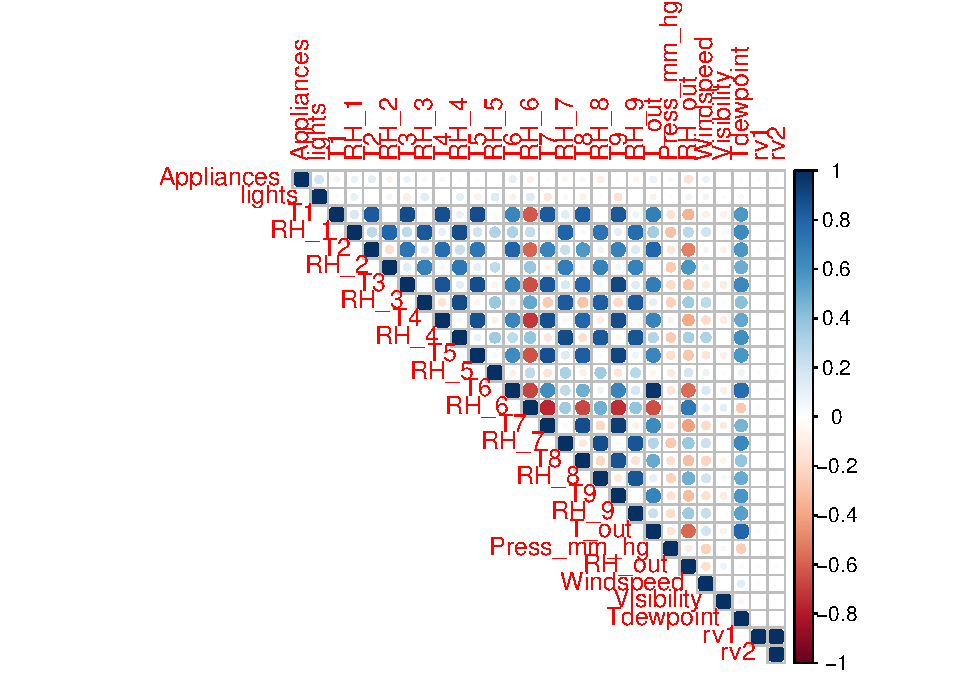
\includegraphics[width=468]{README_figs/README-unnamed-chunk-6-1}

The above plot shows the existing positive and negative correaltions
among the variables. For example there is a negative correlation between
RH\_6 (humidity outside the home) and T7 (tempreture in ironing room).
This plot shows us the way that values of two variables change against
each other, i.e., positive or negative.

\subsubsection{Boxplot}\label{boxplot}

The following boxplot shows the distribution values of T7 over existing
cycles.

\begin{Shaded}
\begin{Highlighting}[]
\CommentTok{#Creating a ts object, we set the frequency to 30, such that box plots shows the distributions per day}
\NormalTok{T7.ts=}\KeywordTok{ts}\NormalTok{(}\KeywordTok{coredata}\NormalTok{(energy_xts[,}\KeywordTok{which}\NormalTok{(}\KeywordTok{names}\NormalTok{(energy_xts) }\OperatorTok{==}\StringTok{ "T7"}\NormalTok{)]), }\DataTypeTok{start=}\DecValTok{1}\NormalTok{, }\DataTypeTok{frequency =} \DecValTok{30}\NormalTok{)}
\KeywordTok{boxplot}\NormalTok{(T7.ts }\OperatorTok{~}\StringTok{ }\KeywordTok{cycle}\NormalTok{(T7.ts))}
\end{Highlighting}
\end{Shaded}

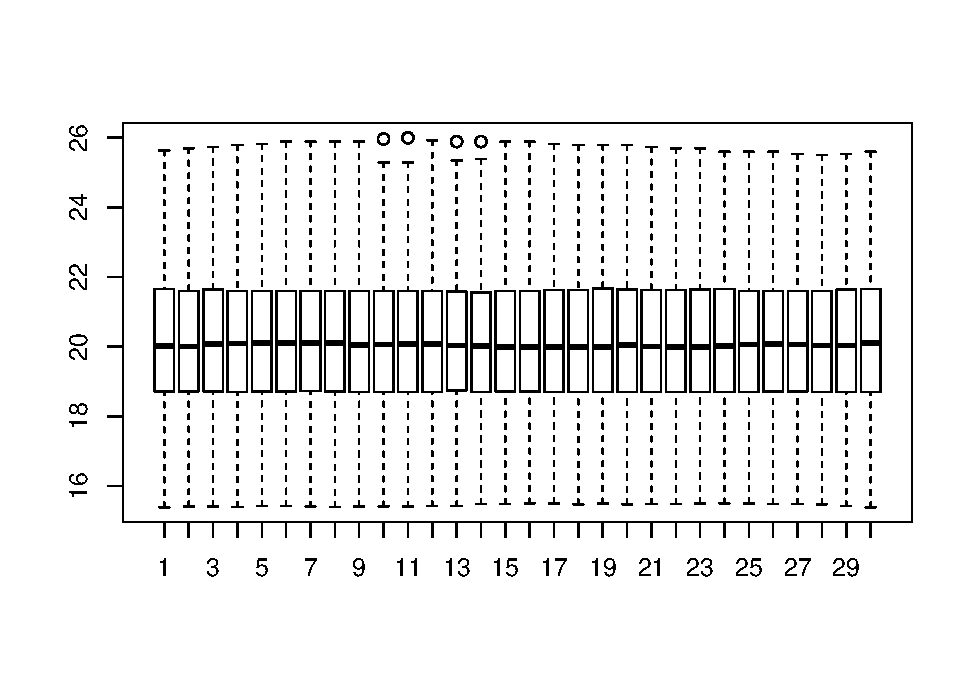
\includegraphics[width=468]{README_figs/README-unnamed-chunk-7-1}

The above plot shows the distributions of temperature for different days
are very similar for the given dataset.

\subsubsection{Histogram}\label{histogram}

One way to identify whether a timeseries is stationary, is to look at
its histogram. Usually bell-shaped histograms can be regarded as
stationary processes, whereas skewed distrobutions show non-stationary
processes.

\begin{Shaded}
\begin{Highlighting}[]
\CommentTok{#Excluding the last two columns since they are not timesereis}
\KeywordTok{multi.hist}\NormalTok{(energy_xts[,}\OperatorTok{!}\KeywordTok{names}\NormalTok{(energy_xts) }\OperatorTok\StringTok{ }\KeywordTok{c}\NormalTok{(}\StringTok{'rv1'}\NormalTok{, }\StringTok{'rv2'}\NormalTok{)])}
\end{Highlighting}
\end{Shaded}

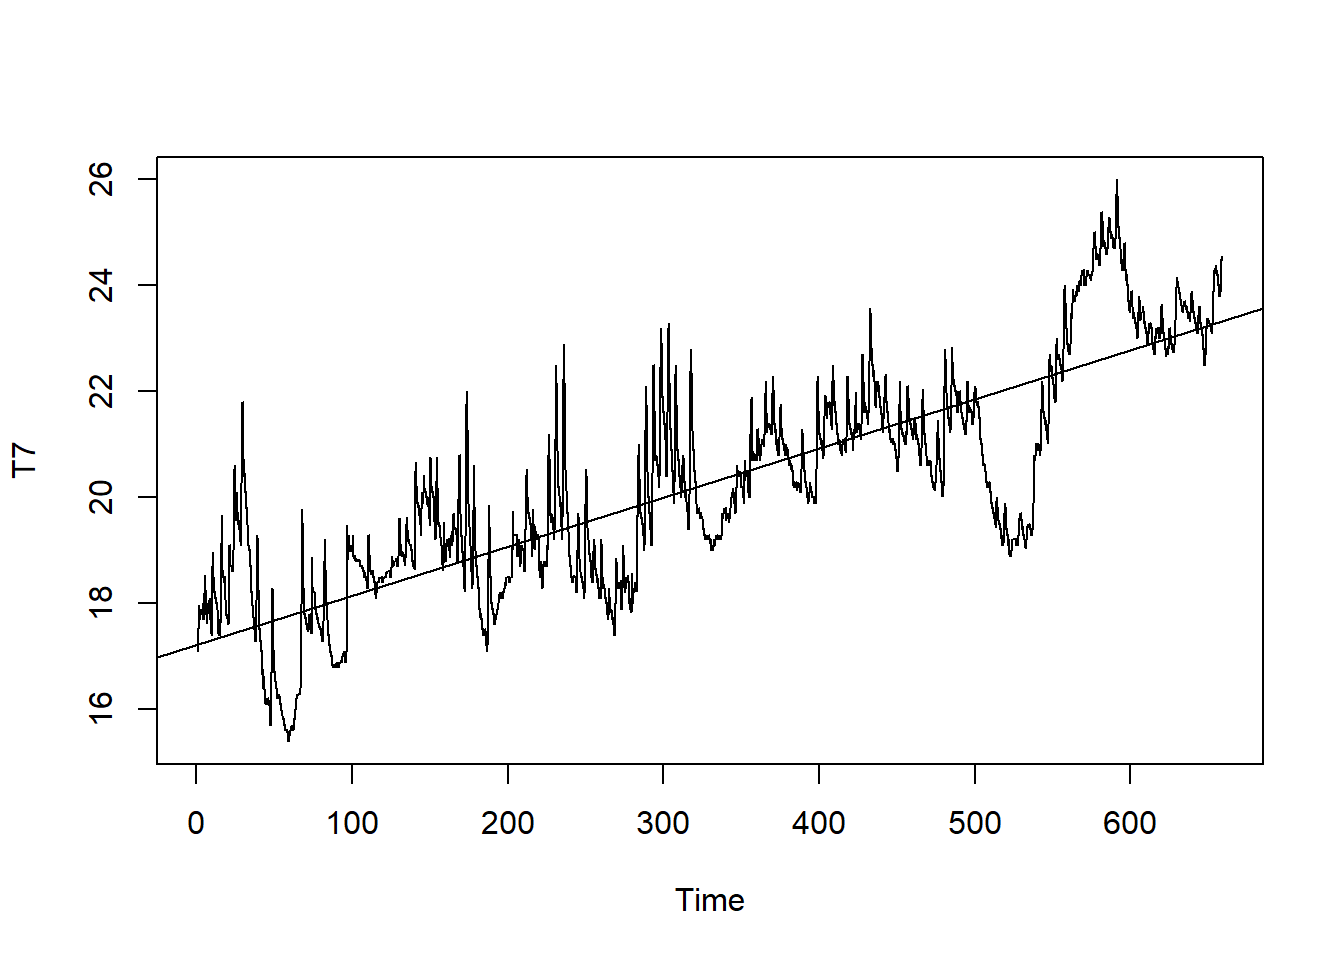
\includegraphics[width=468]{README_figs/README-unnamed-chunk-8-1}

As the above plot shows most of timeseries variables except
\textbf{Windspeed, RH\_out} are stationary.

\subsubsection{Timeseries with Abline}\label{timeseries-with-abline}

Using linear regression, it is easy to see that the trend is increasing;
however, it is not a surprising fact since observations are samples from
January to May and thus temperature increases in this period. More
importantly, the variance of T7 increases as time passes and due to that
the time-series in not stationarity. Above that, one can see that the
variance and mean of T7 increase as time goes by.

\begin{Shaded}
\begin{Highlighting}[]
\KeywordTok{plot}\NormalTok{(T7.ts) }\CommentTok{# plot the raw data}
\KeywordTok{abline}\NormalTok{(}\DataTypeTok{reg=}\KeywordTok{lm}\NormalTok{(}\KeywordTok{coredata}\NormalTok{(T7.ts) }\OperatorTok{~}\KeywordTok{time}\NormalTok{(T7.ts))) }\CommentTok{# fit a trend line}
\end{Highlighting}
\end{Shaded}

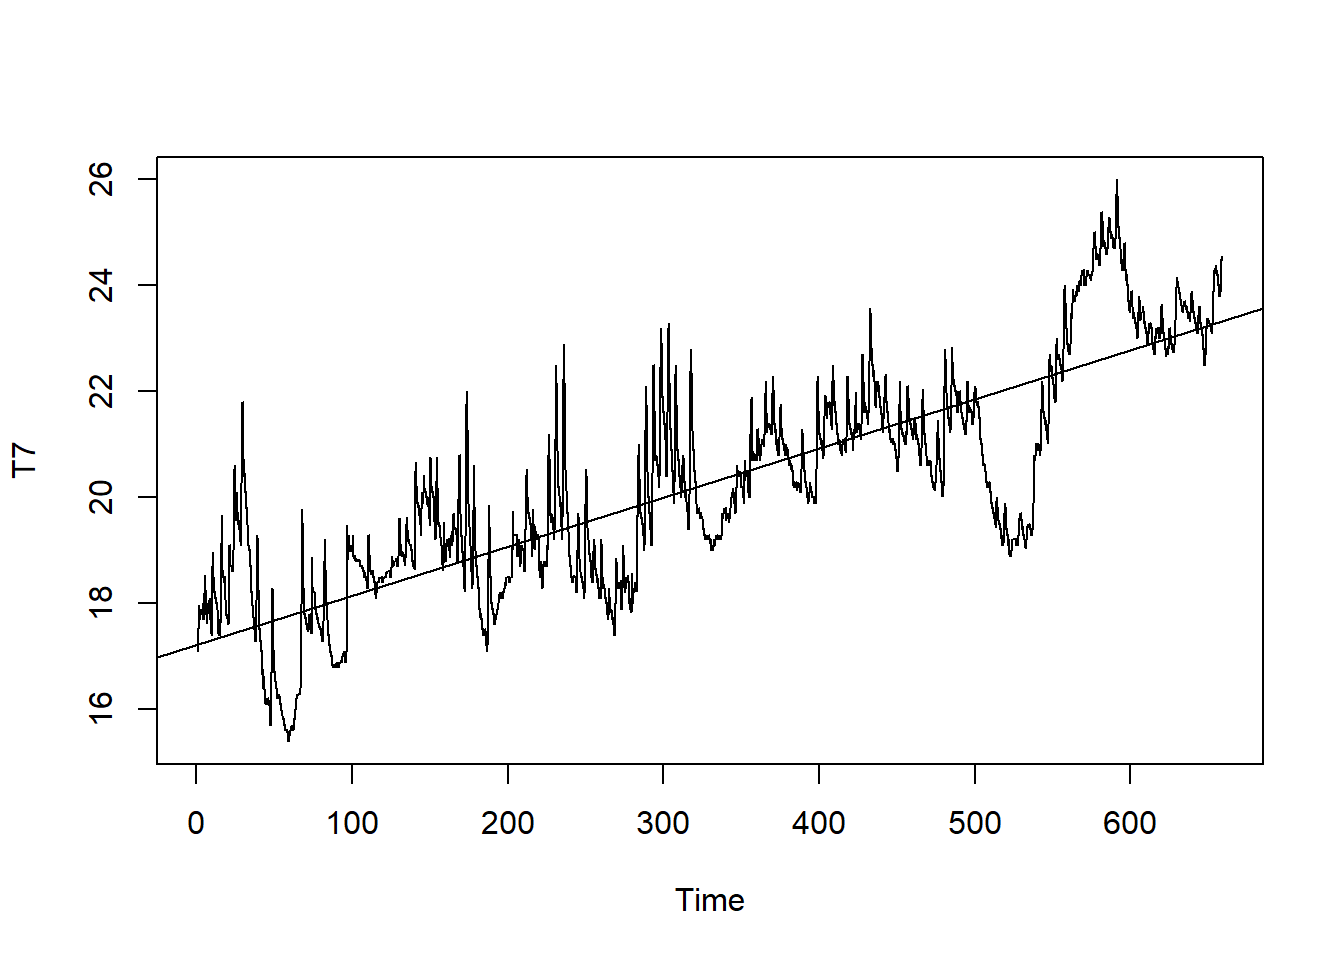
\includegraphics[width=468]{README_figs/README-unnamed-chunk-9-1}

\section{Stationarity}\label{stationarity}

All the previous plots of T7 showed an upward trend which presumably
implies that this time series is not stationary, i.e., corresponding
characteristics change over time. Hence, it must be fixed in some ways.
It can be done by log transformation or by differencing. Each of the
mentioned methods can mitigate to some extent the existing variations
such that, the resulting time series becomes closer to stationarity.

\subsection{Transformation}\label{transformation}

The following codes transfomr T7 into logarithmic and reciprocal values.

\begin{Shaded}
\begin{Highlighting}[]
\CommentTok{#Creating logarithmic and reciprocal transformations}
\NormalTok{T7.log=}\KeywordTok{log}\NormalTok{(energy_xts[,}\KeywordTok{which}\NormalTok{(}\KeywordTok{names}\NormalTok{(energy_xts) }\OperatorTok{==}\StringTok{ "T7"}\NormalTok{)] )}
\NormalTok{T7.recip =}\StringTok{ }\DecValTok{1}\OperatorTok{/}\NormalTok{energy_xts[,}\KeywordTok{which}\NormalTok{(}\KeywordTok{names}\NormalTok{(energy_xts) }\OperatorTok{==}\StringTok{ "T7"}\NormalTok{)]}

\CommentTok{#Merging timeseries into a single object}
\NormalTok{T7.transform=}\KeywordTok{merge.xts}\NormalTok{(T7.log, T7.recip, energy_xts[,}\KeywordTok{which}\NormalTok{(}\KeywordTok{names}\NormalTok{(energy_xts) }\OperatorTok{==}\StringTok{ "T7"}\NormalTok{)])}
\CommentTok{#Providing column names}
\KeywordTok{colnames}\NormalTok{(T7.transform) =}\StringTok{ }\KeywordTok{c}\NormalTok{(}\StringTok{'log'}\NormalTok{, }\StringTok{'reciprocal'}\NormalTok{, }\StringTok{'original'}\NormalTok{)}
\CommentTok{#Plotting}
\KeywordTok{autoplot}\NormalTok{(T7.transform)}
\end{Highlighting}
\end{Shaded}

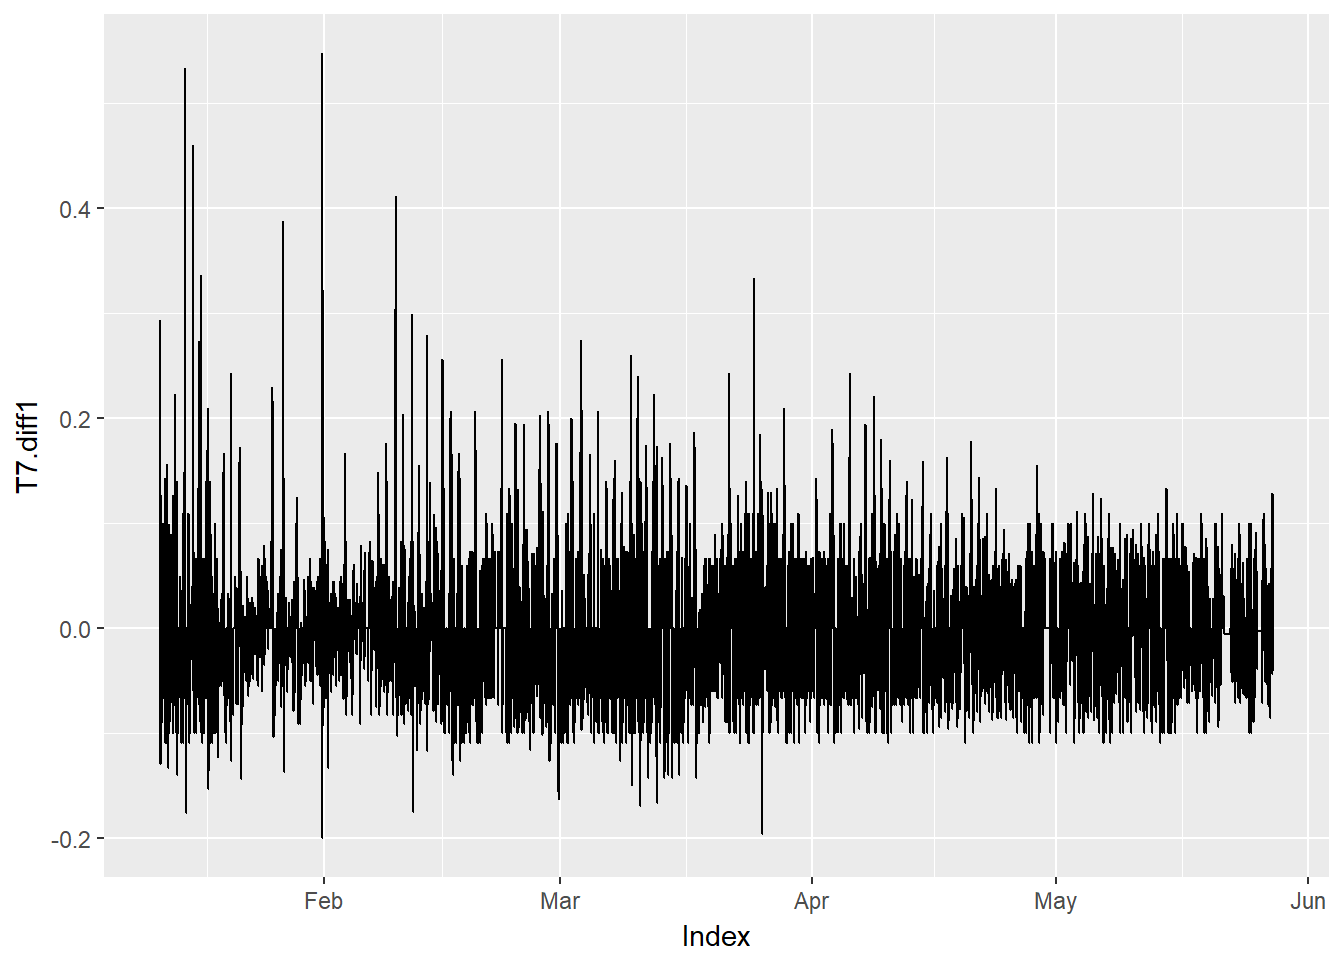
\includegraphics[width=468]{README_figs/README-unnamed-chunk-10-1}

It is clear from the figures that both transformations can make the time
series more stabilize in terms of existing variations. From the figures,
the reciprocal and logarithmic transformations look like a horizontal
line, but it is owing to inappropriate scaling that occurred when three
figures are packed into one frame. Also, it must be stressed that due to
the absence of zero and negative values the mentioned transformations
did work.

Adjusting the correct value of differencing for a timeseries is a brute
force task and there is no shortcuts. In this part, first order
differencing will be adopted to see how it improves the stationary
property of a given time series.

\begin{Shaded}
\begin{Highlighting}[]
\CommentTok{#Creating a first order differencing timeseries}
\NormalTok{T7.diff1=}\KeywordTok{diff}\NormalTok{(energy_xts[,}\KeywordTok{which}\NormalTok{(}\KeywordTok{names}\NormalTok{(energy_xts) }\OperatorTok{==}\StringTok{ "T7"}\NormalTok{)])}
\CommentTok{#Plotting}
\KeywordTok{autoplot}\NormalTok{(T7.diff1)}\OperatorTok{+}\KeywordTok{ylab}\NormalTok{(}\StringTok{"T7.diff1"}\NormalTok{)}
\end{Highlighting}
\end{Shaded}

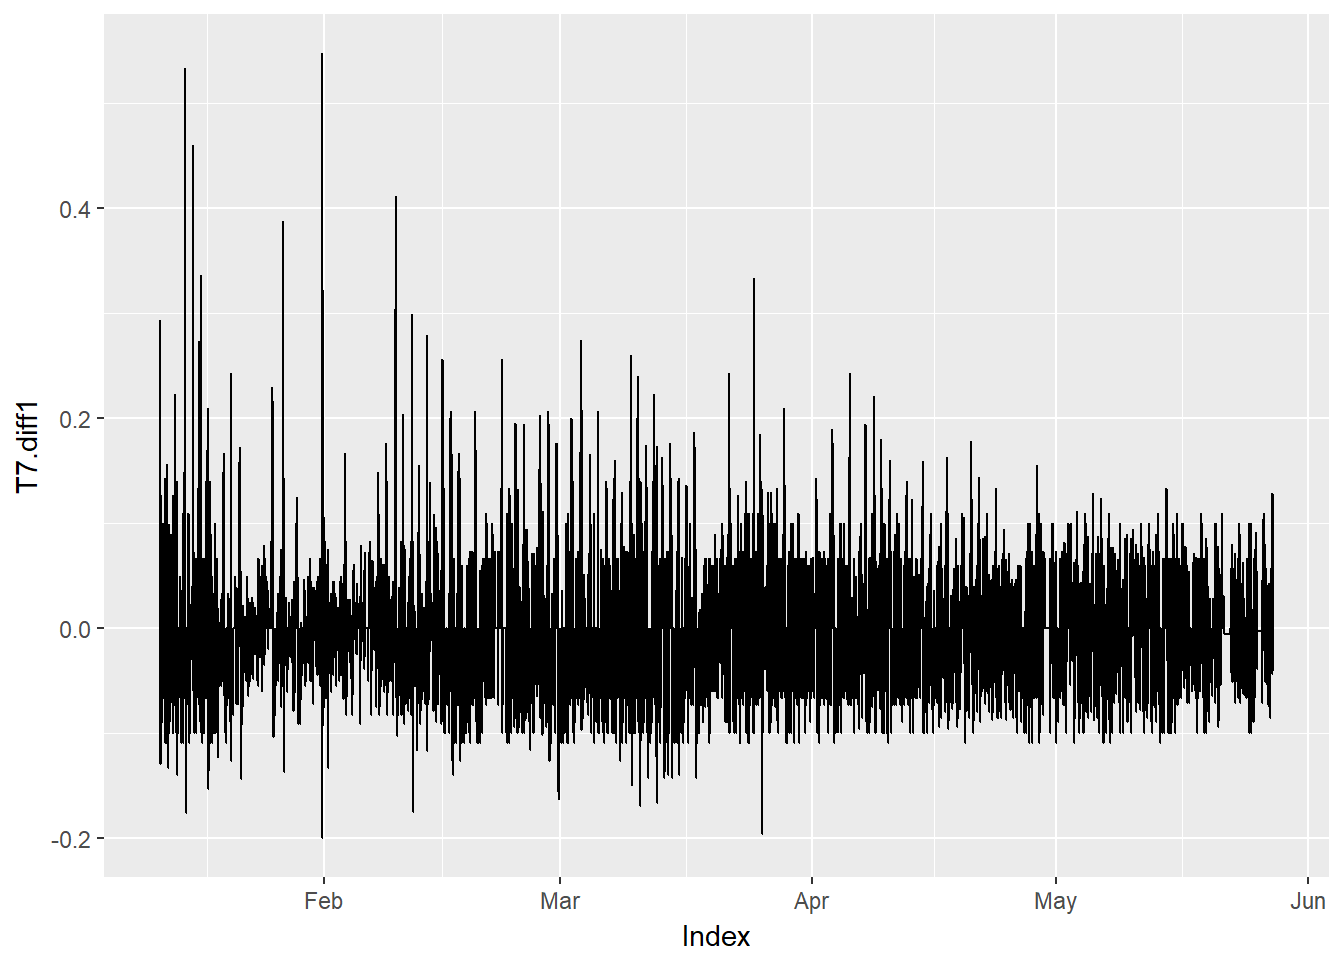
\includegraphics[width=468]{README_figs/README-unnamed-chunk-11-1}

The above plot shows clearly that the first order differencing (d=1) can
capture the available linear trend and makes a stationary time series.
This results also confirmed the output of linear regression obtained
earlier since the linear regression captures the first order linear
trend of a time series.

\subsection{Decomposition}\label{decomposition}

A timeseries can be decomposed into three main elements, i.e., trend,
seasonal and residuals. We selected ``T7'' for this issue (since
``decompose()'' does not work with XTS objects, a ``ts'' object is
created first). The additive decomposition will be used as follows:

\begin{Shaded}
\begin{Highlighting}[]
\CommentTok{#Creating a ts object (In every month we have (30*24*60)/10 = 4320 samples}
\NormalTok{T7.ts=}\KeywordTok{ts}\NormalTok{(}\KeywordTok{coredata}\NormalTok{(energy_xts[,}\KeywordTok{which}\NormalTok{(}\KeywordTok{names}\NormalTok{(energy_xts) }\OperatorTok{==}\StringTok{ "T7"}\NormalTok{)]), }\DataTypeTok{start=}\DecValTok{1}\NormalTok{, }\DataTypeTok{frequency =} \DecValTok{4320}\NormalTok{)}
\CommentTok{#decomposing}
\KeywordTok{plot}\NormalTok{(}\KeywordTok{decompose}\NormalTok{(T7.ts))}
\end{Highlighting}
\end{Shaded}

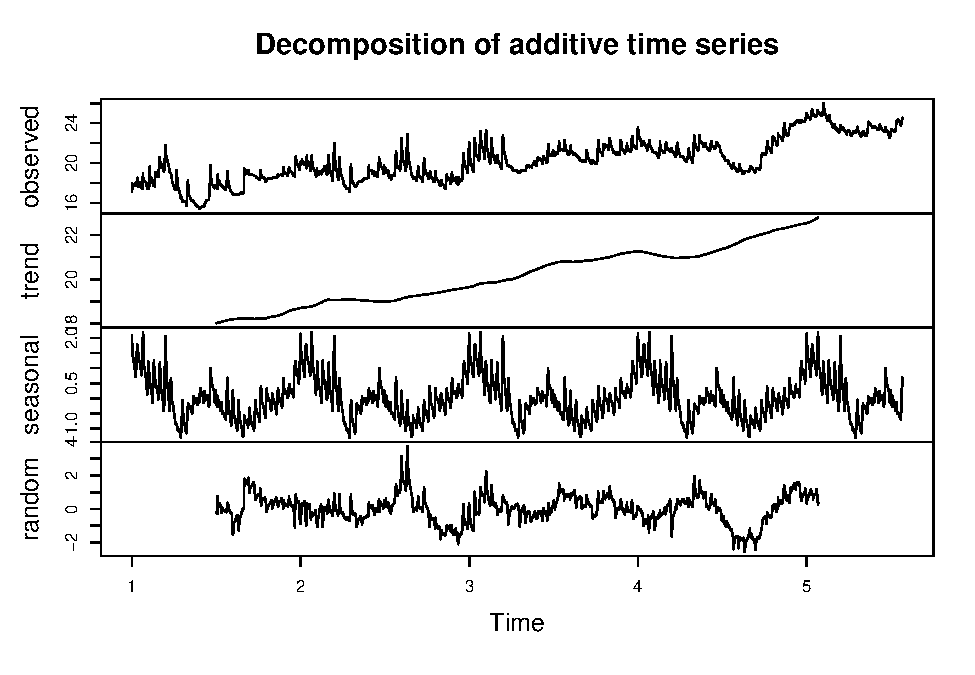
\includegraphics[width=468]{README_figs/README-unnamed-chunk-12-1}

As shown in the above figures, the trend is increasing as it is supposed
to be, since the observations are sampled from January until May. The
seasonal plot clearly depicts cycles in each month. More importantly,
one can see that the ransom noise is fully captured by this
decomposition ( it is random since no specific patterns are observed).

\subsection{Linear Regression}\label{linear-regression}

The linear trend for variable T7 could be obtained via linear regression
as follows. It must be mentioned that a ``ts'' object must be created
first since an ``XTS'' object does not work well with ``lm()'' function.

\begin{Shaded}
\begin{Highlighting}[]
\CommentTok{#Creating a "ts" object for T7}
\NormalTok{T7.ts=}\StringTok{ }\KeywordTok{ts}\NormalTok{(}\KeywordTok{coredata}\NormalTok{(energy_xts[,}\KeywordTok{which}\NormalTok{(}\KeywordTok{names}\NormalTok{(energy_xts) }\OperatorTok{==}\StringTok{ "T7"}\NormalTok{)])[,}\DecValTok{1}\NormalTok{], }\DataTypeTok{start=}\DecValTok{1}\NormalTok{)}
\CommentTok{#Regression with intercept}
\NormalTok{fit.linear=}\KeywordTok{lm}\NormalTok{(T7.ts }\OperatorTok{~}\StringTok{ }\KeywordTok{time}\NormalTok{(T7.ts))}
\CommentTok{#summary of the model}
\KeywordTok{summary}\NormalTok{(fit.linear)}
\NormalTok{## }
\NormalTok{## Call:}
\NormalTok{## lm(formula = T7.ts ~ time(T7.ts))}
\NormalTok{## }
\NormalTok{## Residuals:}
\NormalTok{##     Min      1Q  Median      3Q     Max }
\NormalTok{## -3.1692 -0.7134  0.0900  0.6497  4.3088 }
\NormalTok{## }
\NormalTok{## Coefficients:}
\NormalTok{##              Estimate Std. Error t value Pr(>|t|)    }
\NormalTok{## (Intercept) 1.722e+01  1.653e-02  1041.4   <2e-16 ***}
\NormalTok{## time(T7.ts) 3.092e-04  1.451e-06   213.1   <2e-16 ***}
\NormalTok{## ---}
\NormalTok{## Signif. codes:  0 '***' 0.001 '**' 0.01 '*' 0.05 '.' 0.1 ' ' 1}
\NormalTok{## }
\NormalTok{## Residual standard error: 1.161 on 19733 degrees of freedom}
\NormalTok{## Multiple R-squared:  0.6972, Adjusted R-squared:  0.6972 }
\NormalTok{## F-statistic: 4.543e+04 on 1 and 19733 DF,  p-value: < 2.2e-16}
\CommentTok{#Plot linear trend}
\KeywordTok{ggplot}\NormalTok{(}\DataTypeTok{data=}\KeywordTok{data.frame}\NormalTok{(}\DataTypeTok{real=}\NormalTok{T7.ts, }\DataTypeTok{fit=}\NormalTok{fit.linear}\OperatorTok{$}\NormalTok{fitted.values, }\DataTypeTok{time =} \KeywordTok{time}\NormalTok{(energy_xts[,}\DecValTok{15}\NormalTok{])))}\OperatorTok{+}
\StringTok{  }\KeywordTok{geom_line}\NormalTok{(}\KeywordTok{aes}\NormalTok{(}\DataTypeTok{x=}\NormalTok{time, }\DataTypeTok{y=}\NormalTok{real), }\DataTypeTok{col=}\StringTok{"black"}\NormalTok{) }\OperatorTok{+}\StringTok{ }\KeywordTok{geom_line}\NormalTok{(}\KeywordTok{aes}\NormalTok{(}\DataTypeTok{x=}\NormalTok{time, }\DataTypeTok{y=}\NormalTok{fit), }\DataTypeTok{col=}\StringTok{"blue"}\NormalTok{)}
\end{Highlighting}
\end{Shaded}

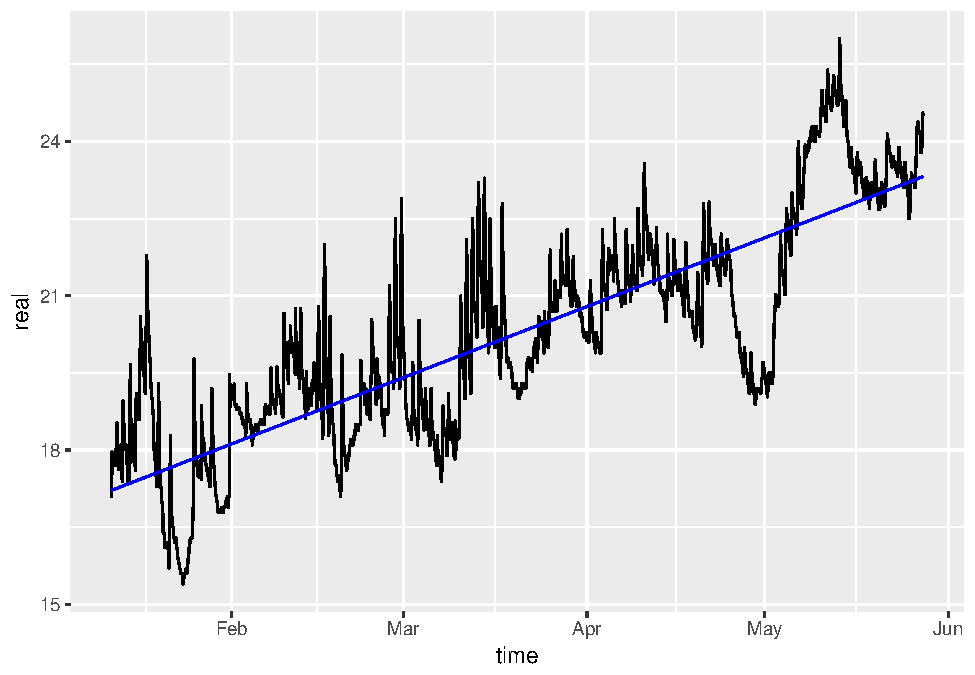
\includegraphics[width=468]{README_figs/README-unnamed-chunk-13-1}

The estimated regression is \(T7 = 0.172 + 0.0003t\). All the
coefficients are statistically significant. The esimtated coffeicient
for the time (t), tells that in each 10 minutes there is an increase
amount of temprature, i.e., \(3.092e-04\), in its unit of measurement.
Also the adjusted \(R^2\) is 0.69, which means that the estimated linear
regression can explain \(69%\) of target variables's variation.

\subsection{Smoohting}\label{smoohting}

Also, a timeseries can be smoothed by different methods to see the
underlying trend. The locally-weighted polynomial regression (lowess)
will be invoked for this matter.

\begin{Shaded}
\begin{Highlighting}[]
\CommentTok{#Smoohting using Lowess for T7}
\NormalTok{T7.lowess=}\KeywordTok{lowess}\NormalTok{(energy_xts[,}\KeywordTok{which}\NormalTok{(}\KeywordTok{names}\NormalTok{(energy_xts) }\OperatorTok{==}\StringTok{ "T7"}\NormalTok{)])}
\CommentTok{#Plotting the time series and its trend}
\KeywordTok{ggplot}\NormalTok{(}\DataTypeTok{data=}\KeywordTok{data.frame}\NormalTok{(}\DataTypeTok{real=}\KeywordTok{coredata}\NormalTok{(energy_xts[,}\DecValTok{15}\NormalTok{])[,}\DecValTok{1}\NormalTok{], }\DataTypeTok{smooth =}\NormalTok{ T7.lowess}\OperatorTok{$}\NormalTok{y, }
                       \DataTypeTok{time=} \KeywordTok{time}\NormalTok{(energy_xts[,}\DecValTok{15}\NormalTok{])))}\OperatorTok{+}
\StringTok{  }\KeywordTok{geom_line}\NormalTok{(}\KeywordTok{aes}\NormalTok{(}\DataTypeTok{x=}\NormalTok{time, }\DataTypeTok{y=}\NormalTok{real), }\DataTypeTok{col=}\StringTok{"black"}\NormalTok{) }\OperatorTok{+}\StringTok{ }\KeywordTok{geom_line}\NormalTok{(}\KeywordTok{aes}\NormalTok{(}\DataTypeTok{x=}\NormalTok{time, }\DataTypeTok{y=}\NormalTok{smooth), }\DataTypeTok{col=}\StringTok{"red"}\NormalTok{)}
\end{Highlighting}
\end{Shaded}

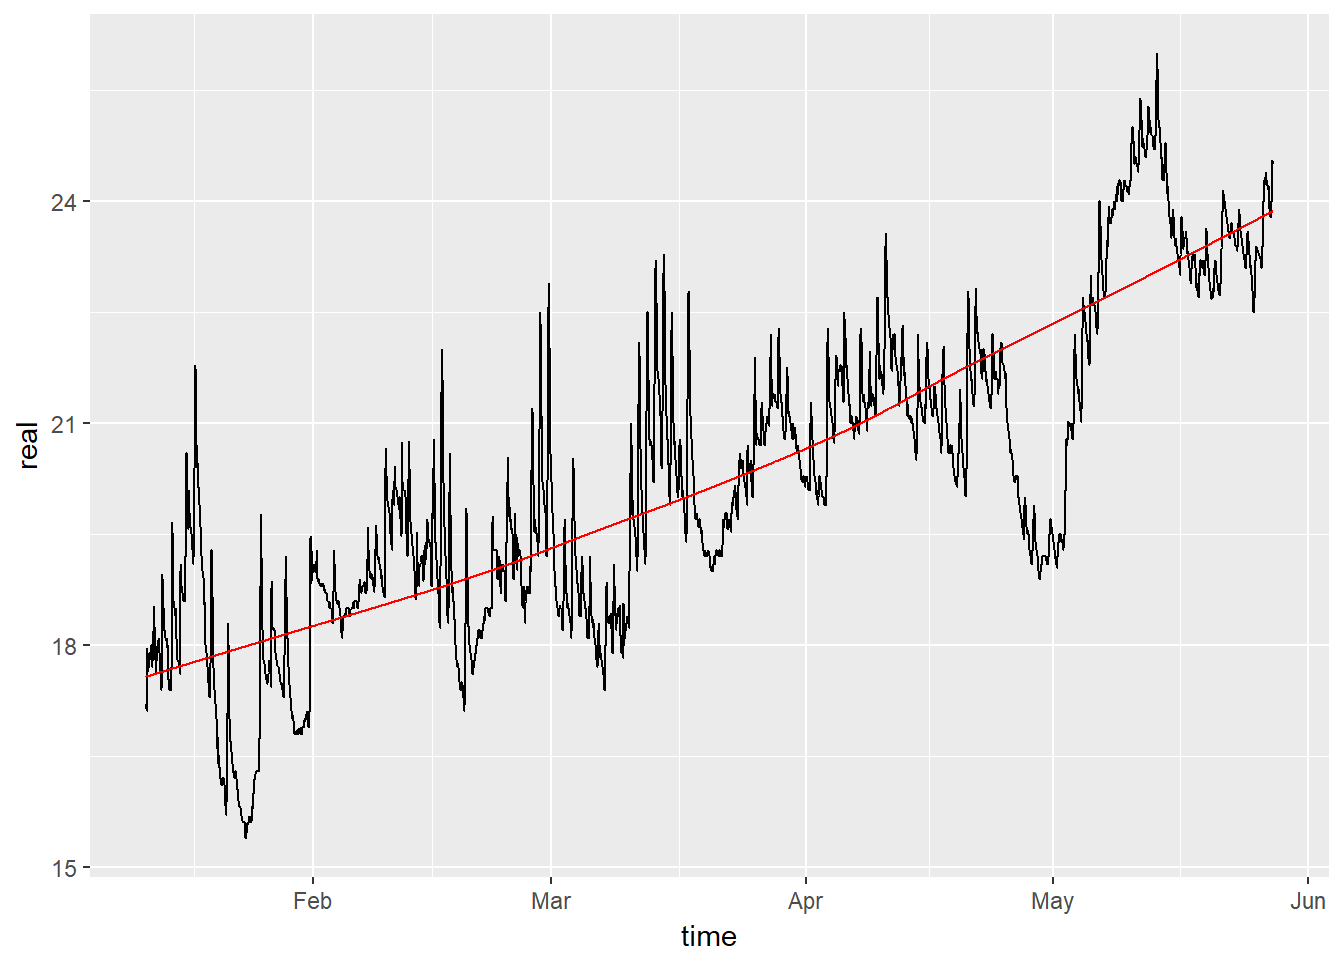
\includegraphics[width=468]{README_figs/README-unnamed-chunk-14-1} The
result shows an upward trend for the variable T7 (temprature in ironing
room), which is not a surprising fact since the timeseries is captured
from spring to summer.

\section{ARMA, ARIMA and Model Diagnostic and
Selection}\label{arma-arima-and-model-diagnostic-and-selection}

A timeseries can be modeled through different formulations, including
Moving Average (MA), Auto Regresive (AR), AutoRegressive Moving Average
(ARMA) and AutoRegressive Integrated Moving Average (ARIMA). Before
getting into the details, it would be helpful to investigate
Autocorrelation Function (ACF) and Partially Autocorrelation Function
(PACF) plots. These plots guide us which model better fits the data
under consideration.

\subsection{ACF and PACF}\label{acf-and-pacf}

This part continues the investigation for timeseries ``T7''. The
following shows corresponding ACF and PACF for this variable.

\begin{Shaded}
\begin{Highlighting}[]
\CommentTok{#Plotting ACF and PACF for T7}
\KeywordTok{acf2}\NormalTok{(energy_xts[,}\KeywordTok{which}\NormalTok{(}\KeywordTok{names}\NormalTok{(energy_xts) }\OperatorTok{==}\StringTok{ "T7"}\NormalTok{)])}
\end{Highlighting}
\end{Shaded}

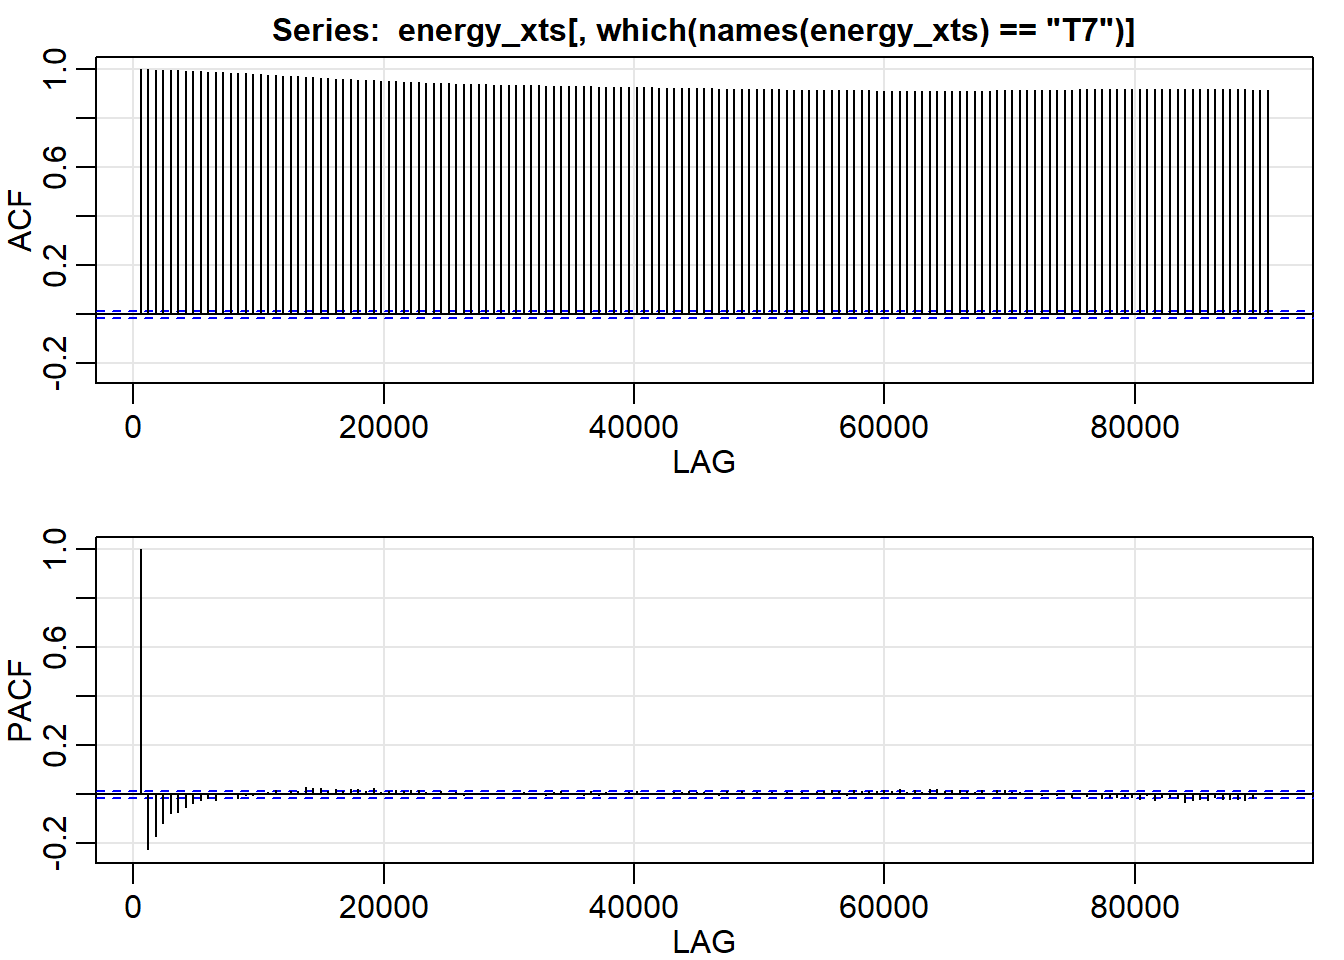
\includegraphics[width=468]{README_figs/README-unnamed-chunk-15-1}

These plots can help us to select the right model's form. Indeed, MA
processes have an ACF plot that is \textbf{cut off} whereas for AR and
ARMA processes it is \textbf{tailed off}. On the other side, PACF can
provide a distinction between ARMA and AR, where, for the former, the
plot is tailed off, and for the later, it is cut off. From the above
plot, It is suspected that the model's form is ARMA since the PACF does
not show a clear cut off (it is gradually decreasing from the second lag
onwards). We can check this issue in another way using AIC information
criterion. Indeed, the AIC criterion tells us which model better fits
the data and have a smaller number of variables. The aim is to build
some models and compares corresponding AIC values.

\subsection{Model Building}\label{model-building}

In this section, different models will be created and compared in terms
of AIC values.

\begin{Shaded}
\begin{Highlighting}[]
\CommentTok{#Creating different models}
\CommentTok{#First order AR}
\NormalTok{AR1=}\KeywordTok{arima}\NormalTok{(energy_xts[,}\KeywordTok{which}\NormalTok{(}\KeywordTok{names}\NormalTok{(energy_xts) }\OperatorTok{==}\StringTok{ "T7"}\NormalTok{)], }\DataTypeTok{order=}\KeywordTok{c}\NormalTok{(}\DecValTok{1}\NormalTok{,}\DecValTok{0}\NormalTok{,}\DecValTok{0}\NormalTok{) )}
\CommentTok{#First order MA}
\NormalTok{MA1=}\KeywordTok{arima}\NormalTok{(energy_xts[,}\KeywordTok{which}\NormalTok{(}\KeywordTok{names}\NormalTok{(energy_xts) }\OperatorTok{==}\StringTok{ "T7"}\NormalTok{)], }\DataTypeTok{order=}\KeywordTok{c}\NormalTok{(}\DecValTok{0}\NormalTok{,}\DecValTok{0}\NormalTok{,}\DecValTok{1}\NormalTok{) )}
\CommentTok{#ARMA(1,0,1)}
\NormalTok{ARMA=}\KeywordTok{arima}\NormalTok{(energy_xts[,}\KeywordTok{which}\NormalTok{(}\KeywordTok{names}\NormalTok{(energy_xts) }\OperatorTok{==}\StringTok{ "T7"}\NormalTok{)], }\DataTypeTok{order=}\KeywordTok{c}\NormalTok{(}\DecValTok{1}\NormalTok{,}\DecValTok{0}\NormalTok{,}\DecValTok{1}\NormalTok{) )}
\CommentTok{#ARIMA(1,1,0)}
\NormalTok{ARIMA=}\KeywordTok{arima}\NormalTok{(energy_xts[,}\KeywordTok{which}\NormalTok{(}\KeywordTok{names}\NormalTok{(energy_xts) }\OperatorTok{==}\StringTok{ "T7"}\NormalTok{)], }\DataTypeTok{order=}\KeywordTok{c}\NormalTok{(}\DecValTok{1}\NormalTok{,}\DecValTok{1}\NormalTok{,}\DecValTok{0}\NormalTok{) )}

\CommentTok{#Comparing AIC values}
\KeywordTok{print}\NormalTok{(}\KeywordTok{cat}\NormalTok{(}\StringTok{"AIC for different models:}\CharTok{\textbackslash{}n}\StringTok{"}\NormalTok{, }\StringTok{"AR1:"}\NormalTok{,}\KeywordTok{round}\NormalTok{(}\KeywordTok{AIC}\NormalTok{(AR1),}\DecValTok{2}\NormalTok{), }\StringTok{"}\CharTok{\textbackslash{}n}\StringTok{ MA1:"}\NormalTok{,}\KeywordTok{round}\NormalTok{(}\KeywordTok{AIC}\NormalTok{(MA1),}\DecValTok{2}\NormalTok{), }
            \StringTok{"}\CharTok{\textbackslash{}n}\StringTok{ ARMA:"}\NormalTok{, }\KeywordTok{round}\NormalTok{(}\KeywordTok{AIC}\NormalTok{(ARMA),}\DecValTok{2}\NormalTok{), }\StringTok{"}\CharTok{\textbackslash{}n}\StringTok{ ARIMA:"}\NormalTok{, }\KeywordTok{round}\NormalTok{(}\KeywordTok{AIC}\NormalTok{(ARIMA),}\DecValTok{2}\NormalTok{) ))}
\NormalTok{## AIC for different models:}
\NormalTok{##  AR1: -67703.44 }
\NormalTok{##  MA1: 58587.65 }
\NormalTok{##  ARMA: -69806.58 }
\NormalTok{##  ARIMA: -70917.15NULL}
\end{Highlighting}
\end{Shaded}

As shown by AIC values above, ARIMA has better ability to fit data
(smaller AIC value), but instead of finding the parameters of this model
in an exhaustive way, we can resort to ``Auto.arima()'' function that
returns the most fitting model.

\begin{Shaded}
\begin{Highlighting}[]
\CommentTok{#Fitting the best model }
\NormalTok{Best.fit=}\KeywordTok{auto.arima}\NormalTok{(energy_xts[,}\KeywordTok{which}\NormalTok{(}\KeywordTok{names}\NormalTok{(energy_xts) }\OperatorTok{==}\StringTok{ "T7"}\NormalTok{)])}
\KeywordTok{summary}\NormalTok{(Best.fit)}
\NormalTok{## Series: energy_xts[, which(names(energy_xts) == "T7")] }
\NormalTok{## ARIMA(1,1,1) }
\NormalTok{## }
\NormalTok{## Coefficients:}
\NormalTok{##          ar1      ma1}
\NormalTok{##       0.9066  -0.6740}
\NormalTok{## s.e.  0.0049   0.0086}
\NormalTok{## }
\NormalTok{## sigma^2 estimated as 0.001452:  log likelihood=36475.42}
\NormalTok{## AIC=-72944.85   AICc=-72944.85   BIC=-72921.18}
\NormalTok{## }
\NormalTok{## Training set error measures:}
\NormalTok{##                        ME       RMSE        MAE          MPE      MAPE}
\NormalTok{## Training set 0.0001068284 0.03810826 0.02321765 0.0007849972 0.1151972}
\NormalTok{##                     MASE         ACF1}
\NormalTok{## Training set 0.001145583 -0.004181521}
\KeywordTok{AIC}\NormalTok{(Best.fit)}
\NormalTok{## [1] -72944.85}
\end{Highlighting}
\end{Shaded}

The above results indicate the form and parameters of the model which is
ARIMA(1,1,1), i.e., first order difference - autoregressive - moving
average, which confirmes our previous results obtained manually. Also,
one could note that the reported AIC value is smaller than other AIC
values obtained earlier.

To see how good the model is, we will examine the residuals of the
model.

\begin{Shaded}
\begin{Highlighting}[]
\CommentTok{#Plotting residuals}
\KeywordTok{autoplot}\NormalTok{(}\KeywordTok{residuals}\NormalTok{(Best.fit))}
\end{Highlighting}
\end{Shaded}

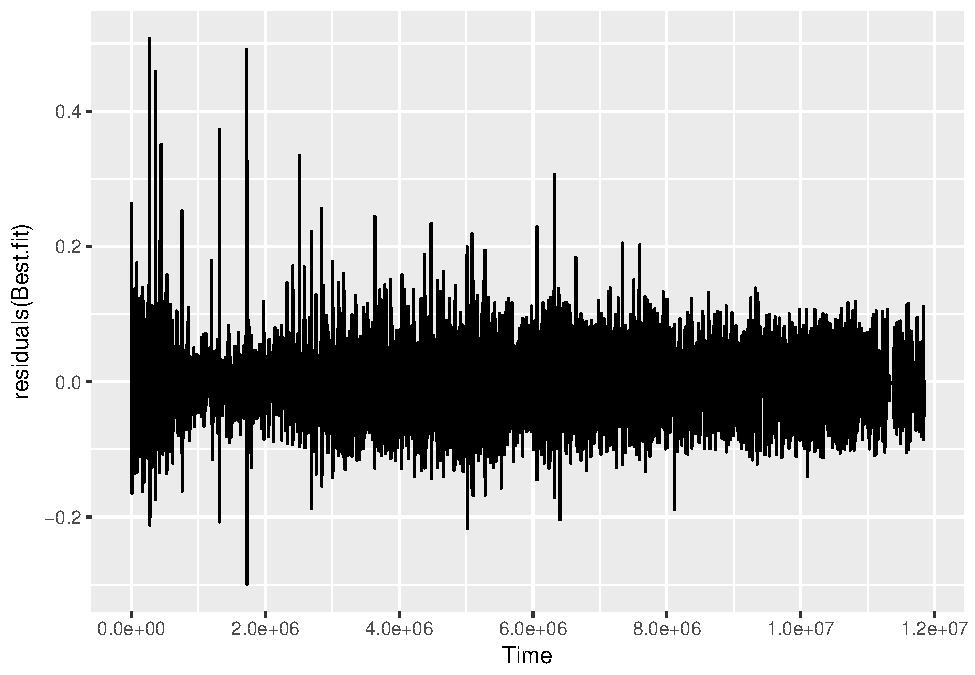
\includegraphics[width=468]{README_figs/README-unnamed-chunk-18-1}

\begin{Shaded}
\begin{Highlighting}[]

\CommentTok{#Further investigations}
\KeywordTok{checkresiduals}\NormalTok{(Best.fit)}
\end{Highlighting}
\end{Shaded}

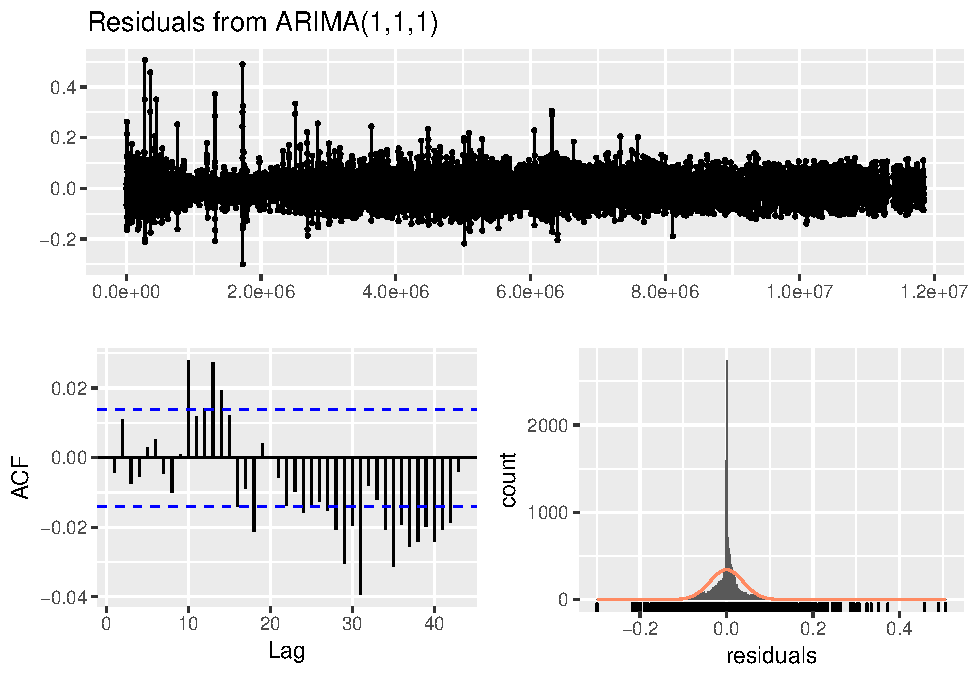
\includegraphics[width=468]{README_figs/README-unnamed-chunk-18-2}

\begin{verbatim}
## 
##  Ljung-Box test
## 
## data:  Residuals from ARIMA(1,1,1)
## Q* = 22.925, df = 8, p-value = 0.003462
## 
## Model df: 2.   Total lags used: 10
\end{verbatim}

Above plots suggest that residuals are normally distributed with mean
zero, constant variance, and there are no specific patterns. However,
residuals are serially correlated, as this fact can be obtained from the
corresponding ACF plot and the results of Ljung-Box test.


\end{document}
